\section{Introducción}
\noindent Sea un conjunto de datos obtenidos de observar ciertas variables aleatorias de manera simultánea. De ese conjunto de variables se dividirán en:
\begin{itemize}
\item \textbf{\textit{Variables de entrada o inputs}}: Son las variables independientes que determinarán de manera aleatoria al segundo conjunto de variables. Al conjunto de variables aleatorias de entrada se la denotará como el vector aleatorio $\textbf{x}^T=[X_1,\ldots X_p]$. \\
Tomando $n$ observaciones de estas variables se obtiene la \textit{matriz de datos} $\textbf{X}$. Esta matriz es de tamaño $n\times p$ y contiene como filas los vectores de longitud $p$ que representan los datos de cada observación, se denotan como $\textbf{x}_i$. Por ejemplo, en el caso de que se recojan datos sobre distintos modelos de coches serían la potencia del motor, el tipo de combustible $etc\ldots$
\item \textbf{\textit{Variables de salida u outputs}}: Son las variables dependientes de las anteriores. A este conjunto de variables se les denota con el vector aleatorio $\textbf{y}^T=[Y_1,\ldots Y_k]$, en el caso de que se tenga una única variable respuesta se denotará como $Y$. \\
Como en el caso de las variables de entrada, se tomarán $n$ observaciones de las $k$ variables, dando como resultado la matriz de respuestas $\textbf{Y}$ de tamaño $n \times k$, donde cada observación es una fila y se denota como $\textbf{y}_i$, en el caso de que $k>1$ y como $y_i$ cuando $k=1$. Siguiendo el ejemplo anterior, se podrían tener variables respuesta como el tipo de etiqueta medioambiental siendo esta una variable cualitativa o el precio del vehículo que tiene naturaleza cuantitativa. 
\end{itemize}
\noindent Por ende, se recogen observaciones simultáneas de las variables de entrada y de salida formando parejas $(\textbf{y}_i,\textbf{x}_i)$. El objetivo de estos métodos supervisados es encontrar una relación funcional o predictor de tal manera que para una nueva observación de las variables de entrada $\textbf{x}_0$ se pueda hacer una predicción $\hat{\textbf{y}}_0$ del valor real $\textbf{y}_0$ de la variable respuesta. 
 
\subsection{Mínimos cuadrados y K-vecinos más cercanos}
\noindent Supóngase el caso en el que únicamente tenemos una variable respuesta $Y$. Además supóngase que la relación que se utiliza para realizar predicciones  $\hat{y}$ de los valores respuesta es una combinación lineal de los valores predictores, de manera que se tiene un vector $\hat{\beta}=[\hat{\beta}_0,\ldots,\hat{\beta}_p]$ de parámetros que permite hacer predicciones de la siguiente manera para una nueva observación $\textbf{x}_0$:
\begin{equation}
\hat{y}_0=\hat{\beta}_0+ \sum_{j=1}^p \hat{\beta}_j x_{0j}
\end{equation}

\noindent Utilizando una primera componente de $\textbf{x}_0$ igual a 1 se puede dar la expresión como producto matricial.
\begin{equation}
\hat{y}_0=\textbf{x}_0^T \hat{\beta}
\end{equation}

\noindent Para este y muchos otros casos el modelo ha de ajustarse a los datos recogidos para las $p$ variables de entrada y las variables respuesta que se tengan en ese momento. Para poder dar una medida de la calidad del ajuste se definen las funciones de pérdida. 
\begin{defi}
Se llama \textit{función de pérdida} a la función que cuantifica el error cometido al usar la predicción y se denota como $L(y,\hat{y})$
\end{defi} 

\noindent Si se toma como medida global la suma de las pérdidas de todas las observaciones, en el caso de que $L(y,\hat{y})=(y-\hat{y})^2$ se obtiene el \textit{Error Cuadrático Acumulado} o \textit{RSS} por su siglas en inglés. 
\begin{defi}
Se define el \textit{Error Cuadrático Acumulado} a la suma de los cuadrados de las diferencias entre las predicciones y los valores reales de la variable respuesta. En el caso de una sola variable aleatoria respuesta y suponiendo que se han recogido $n$ observaciones conjuntas se expresa de la siguiente manera: 
\begin{align}
RSS=\sum_{i=1}^n L(y_i,\hat{y}_i)&=\sum_{i=1}^n (y_i-\hat{y}_i)^2
\intertext{ para el caso del modelo lineal: } RSS(\beta)=\sum_{i=1}^n (y_i-\hat{y}_i)^2&=\sum_{i=1}^n (y_i-\textbf{x}_i^T \beta)^2
\end{align}
\end{defi}
\noindent En esencia, este error cuadrático acumulado no es más que la pérdida total del conjunto de datos. Esto nos da una forma de la calidad global del ajuste. Además es generalizable a otras funciones de pérdida. 

\noindent Para ajustar los parámetros $\beta$, se busca minimizar la cantidad de error que se comete al predecir, por tanto, establecemos el problema de optimización con la función $RSS(\beta)$ como función objetivo. Es por ello, que esta debe ser derivable y aunque sea posible elegir otras funciones de pérdida, como pudiera ser $L(y,\hat{y})=\vert y-\hat{y}\vert$, estas resultan en funciones de pérdida globales no derivables. 

\noindent La expresión de $RSS(\beta)$ en forma matricial teniendo en cuenta que $\textbf{X}$ sea la matriz de observaciones de tamaño $(n\times p+1)$ que tiene la primera columna constante 1 e $\textbf{y}$ es el vector columna o matriz que contiene las observaciones de la o las variables respuestas es la siguiente: 
\begin{equation}
RSS(\beta)=(\textbf{y}-\textbf{X}^T\beta)^T(\textbf{y}-\textbf{X}^T\beta)
\end{equation}
Que al derivarla respecto de $\beta$ e igualarlo a $0$ se obtiene que:
\begin{equation}
\textbf{X}^T(\textbf{y}-\textbf{X}\beta)=0
\end{equation}
Que tiene solución única si la matriz $\textbf{X}^T\textbf{X}$ es invertible resultando en que $\hat{\beta}=(\textbf{X}^T\textbf{X})^{-1}\textbf{X}^T\textbf{y}$.

\noindent Este método de ajuste de los parámetros de la función de predicción se llama método de los \textit{Mínimos Cuadrados}, que es de largo el más utilizado aunque tiene sus problemas. 

\noindent Mientras que el modelo (la relación que se usa como predicción) que se ha utilizado asume una cierta estructura global, que tiene sus desventajas, también se pueden dar métodos que no se centren en la estructura a nivel global, sino local. 

\noindent Con este objetivo se construirá uno de los predictores locales más simples y conocidos el método de $k$-vecinos. 

\begin{defi}
Sea un conjunto de $n$ observaciones $\textbf{x}_i, i =1,\ldots n$, se define el conjunto $N_k(\textbf{x}_0)$ al conjunto de las $k$ observaciones más cercanas al punto $\textbf{x}_0$.
\end{defi}

\noindent Una vez definido ese conjunto se puede definir el siguiente predictor: 
\begin{equation}
\hat{y}(\textbf{x}_0)=\dfrac{1}{k}\sum_{\textbf{x}_i\in N_k(\textbf{x}_0)}y_i
\end{equation}

\noindent Este método de predicción no requiere que se realice el ajuste de ningún parámetro (\textit{es un predictor no paramétrico}) y además es bastante simple de utilizar, basta con promediar los valores respuesta de cada una de las observaciones del conjunto de datos. 

\noindent En contraste, el método de los K-Vecinos y los métodos locales en general, sufren de lo que se llama la \textit{maldición de la dimensionalidad}. Este suceso consiste en que a medida que aumentamos la dimensión, en este caso la cantidad de variables aleatorias a observar, la densidad de los datos es cada vez menor. Esto provoca que por ejemplo que los conjuntos $N_k$ sean conjuntos muy dispersos, por tanto las observaciones que usamos como referencias y la observación de la cual se va a realizar la predicción están muy lejanas.\\
En particular, la densidad es proporcional a $n^{\frac{1}{p}}$, donde $p$ es el número de variables y $n$ el número de observaciones. Por ejemplo, si una muestra densa en $1$ dimensión tiene $n=100$, para mantener dicha densidad en $p=10$ se necesitarían $n = 100^{10}$. 
De las características de los espacios de observaciones de altas dimensiones se habla en \textit{Koppen,}\cite{Koppen 2000}

\subsection{Decisión Estadística}
\noindent Sea un vector aleatorio real de entrada $\textbf{x}\in\mathbb{R}^p$, una variable de salida $Y\in\mathbb{R}$ y sea la probabilidad conjunta $\mathbb{P}(Y,\textbf{x})$ de ambas, entonces se busca una función $f(\textbf{x})$ para predecir $Y$, es decir, $\hat{Y}=f(\textbf{x})$. Para ello, se utilizan las funciones de pérdida, en lo sucesivo utilizaremos la pérdida cuadrática $L(Y,\hat{Y})=L(Y,f(\textbf{x}))=(Y-f(\textbf{x}))^2$. 
\begin{defi}
Teniendo en cuenta lo anterior, se define el \textit{error de predicción esperado} como la esperanza de la nueva variable que define la función de pérdida.
\begin{equation}
\begin{split}
EPE(f)& = E(Y-f(\textbf{x}))^2\\
&= \int [y-f(\textbf{x})]^2\mathbb{P}(dx,dy)
\end{split}
\end{equation}
\end{defi}

\noindent Para ajustarlo a la situación de predecir el valor de $Y$ para nuevos valores observados de $\textbf{x}$, se puede condicionar respecto del valor de $\textbf{x}$ obteniendo la siguiente expresión:
\begin{equation}
 EPE(f) = E_{\textbf{x}} E_{Y|\textbf{x}}([Y-f(\textbf{x})]^2|\textbf{x})
\end{equation} 
Esta expresión otorga según \textit{Hastie et.al} \cite{Hastie 2001} un criterio para elegir la $f$. Basta con tomar $f$ de manera que: 
\begin{equation}
 f(x)=\text{argmin}_c E_{Y|\textbf{x}}([Y-c]^2|\textbf{x}=x)
\end{equation}

\noindent Por tanto, el que minimiza en el caso de la pérdida establecida anteriormente es $f(x)=E(Y|\textbf{x}=x)$. 
\begin{defi}
\noindent Se llama \textit{función de regresión} a la función $f(x)=E(Y|\textbf{x}=x)$
\end{defi}

\noindent Por ejemplo, para el caso del modelo de K-Vecinos, la función de regresión es la siguiente:
\begin{equation}
\hat{f}(\textbf{x})=\dfrac{1}{k}\sum_{\textbf{x}_i\in N_k(\textbf{x})} y_i 
\end{equation}

\noindent Hasta ahora, solo se han contemplado los casos en los que la variable respuesta era cualitativa. Para el caso en el que esta sea categórica, la mayoría de conceptos son análogos con ciertas modificaciones.

\noindent Sea el caso de una variable de salida categórica $G$ que toma $k$ valores de manera que el predictor $\hat{G}$ tambien toma esos valores, entonces la única modificación que debemos hacer es la de la función de pérdida que pasa a ser una matriz $\textbf{L}$ de tamaño $k\times k $ donde $L_{i,j}$ es la penalización por categorizar como $\mathcal{G}_j$ algo que en realidad es $\mathcal{G}_i$. Entonces tenemos que \textit{el error de predicción esperado} es: 
\begin{equation}
EPE = E[L(G,\hat{G})]= E_{\textbf{x}}\sum_{i=1}^k L[\mathcal{G}_k, \hat{G}(\textbf{x})]\mathbb{P}(\mathcal{G}_k|\textbf{x})
\end{equation} 
Esta definición otorga un criterio análogo para establecer el predictor $\hat{G}(x)$, que si se utiliza la pérdida 0-1, es decir, aquella que otorga una penalización de 1, se obtiene el \textit{clasificador bayesiano}.
\begin{defi}
Se llama \textit{clasificador bayesiano} al predictor 
\begin{equation}
\hat{G}(x)=\mathcal{G}_k \text{ si } \mathbb{P}(\mathcal{G}_k|\textbf{x}=x)=\max_{g\in \mathcal{G}}\mathbb{P}(g|\textbf{x}=x)
\end{equation}

\noindent Es decir, se otorga la categoría que más probabilidad de ser tiene conociendo el valor de $\textbf{x}$.
\end{defi}

\noindent Una vez definidos los principales predictores, hay que tener en cuenta que este tipo de métodos se pueden ver desde el prisma de un problema de aprendizaje automático, en particular, son métodos de aprendizaje supervisado.

\noindent En este caso, no se detallará como un problema de aprendizaje automático aunque varios métodos de los detallados frecuentemente se interpreten de esta manera. 

\noindent Otra manera es interpretarlo cómo un problema de aproximación de funciones, de manera que se aproximen teniendo en cuenta los puntos $\textbf{x}_i$ en $\mathbb{R}^p$, por ejemplo, en el caso del modelo lineal se intenta ajustar un hiperplano afín. 

\noindent Aún así, a estos métodos se les llama \textit{métodos supervisados} ya que se parte del conocimiento de las observaciones $(\textbf{x}_i,\textbf{y}_i)$ y se adapta el modelo y los parámetros conociendo el valor real de las observaciones de la variable respuesta. 

\subsection{Sesgo y Varianza del Modelo}

\noindent A la hora de elegir un modelo, hay que tener en cuenta la complejidad del mismo, ya que un modelo demasiado complejo puede ajustarse perfectamente a los datos de entrenamiento, pero tener una capacidad de generalización nula. Por otro lado, un modelo demasiado simple puede no captar las características básicas de los datos. 

\noindent Supóngase que la variable respuesta sigue la siguiente expresión $Y=f(\textbf{x})+\varepsilon$ donde $\mathbb{E}(\varepsilon)=0$ y $Var(\varepsilon)=\sigma^2$, supongamos además que las observaciones $\textbf{x}_i$ son ya conocidas. Entonces, se puede expresar el error de predicción de una nueva observación $\textbf{x}_0$ de la siguiente manera:
\begin{equation}
\begin{split}
EPE(\textbf{x}_0)&=\mathbb{E}[(Y-\hat{f}(x))^2|X=\textbf{x}_0]=\\
&=\sigma^2+B^2(\hat{f}(\textbf{x}_0))+Var(\hat{f}(\textbf{x}_0))
\end{split}
\end{equation}

\noindent Esta expresión está compuesta de dos términos que dependen de la estimación, $\hat{f}$, que son el sesgo y la varianza de esta. Ahora bien, hay un término que no depende de la estimación que es $\sigma^2$, el término de error inevitable. 

\noindent Por ejemplo, el modelo de K-Vecinos más cercanos, la complejidad está influida por el parámetro K. Cuántos más vecinos tenga el vecindario, mayor es el sesgo del predictor, ya que entran en juego más observaciones para calcular el valor de $y_i$ y menor es la varianza.  

\noindent La siguiente gráfica ha sido extraída de \textit{Hastie et. al. } \cite{Hastie 2001} y representa el error de predicción en función de la complejidad del modelo. La línea azul es el error de predicción sobre muestras del conjunto de entrenamiento y la roja sobre muestras nuevas que no han sido utilizadas para el ajuste. 

\begin{figure}[h]
\centering
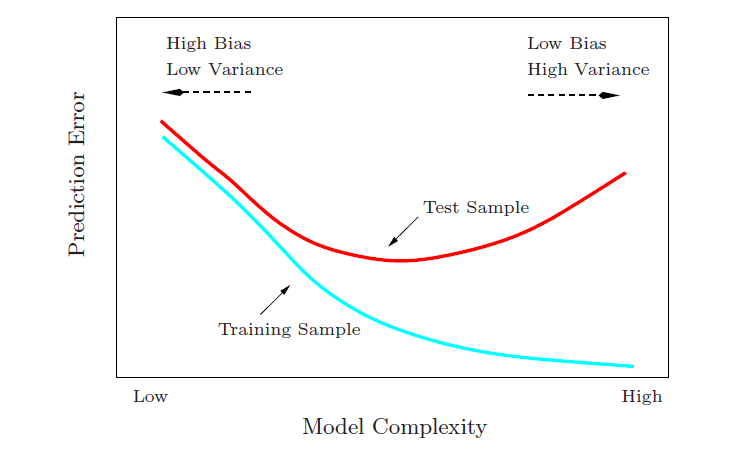
\includegraphics[scale=0.45]{Documentos Extra/Imagenes/Bias-Variance-Tradeoff.png}
\end{figure}
\newpage
\noindent Hay un punto de equilibrio, en el cual una complejidad media otorga un error de predicción aceptable sobre muestras de entrenamiento y un error de predicción no muy alto sobre muestras que no lo son. Cuando se toma modelos demasiado complejos el modelo puede sufrir de \textit{sobreajuste}

\begin{defi}
Se dice que un predictor o modelo sufre de \textit{overfitting} o \textit{sobreajuste} en los casos en los que el predictor tiene un bajo sesgo pero una varianza alta. Esto se ve reflejado en un muy buen ajuste en el conjunto de entrenamiento pero una calidad de predicción de nuevos datos mala. 
\end{defi}

\noindent Estos casos de overfitting se dan por ejemplo, cuando tenemos un conjunto de datos con más variables observadas que observaciones. Hay distintos métodos para evitar el sobreajuste en conjuntos de datos con pocas observaciones, estos se detallan en el capítulo 7 de \textit{Hastie et.al.}\cite{Hastie 2001}





















%\noindent Una característica que se puede intuir es que el problema de encontrar el predictor se puede traducir como un problema de aproximación de funciones en $\mathbb{R}^p$ conocidos $n$ puntos.































%\noindent Teniendo en cuenta lo anterior, y tomando que $f(x)=E(Y|\textbf{x}=x)$ supongamos que los datos vienen dados según el modelo:
%\begin{equation}
%Y = f(\textbf{x})+\varepsilon
%\end{equation}
%Donde la variable aleatoria $\varepsilon$ reúne todos los valores que no estén reunidos bajo las mediciones de las variables del vector aleatorio $\textbf{x}$ y los errores de medición.
%En particular, la variable $\varepsilon$ es independiente de $\textbf{x}$ y $E(\varepsilon)=0$.
%
%Este \textit{modelo aditivo} es una buena representación para la  mayoría de situaciones, y en caso de que no se dé la suposición de la independencia tomando 




%\subsection{Selección del modelo, Sesgo y Varianza}
%
%Una vez que hemos ajustado el modelo a los puntos hay que comprobar su rendimiento, esto se puede hacer teniendo un conjunto de entrenamiento y otro de testing. El conjunto de entrenamiento nos servirá para optimizar los parámetros y el de testing del cual conocemos las x y las y nos permite evaluar su capacidad de generalización. 
%
%\noindent Sea el modelo $Y=f(\textbf{x})+\varepsilon$ donde $E(\varepsilon)=0$ y $Var(\varepsilon)=\sigma^2$. Entonces podemos hacer la siguiente descomposición del error de generalización  esperado en $x_0$, no perteneciente al conjunto de entrenamiento:
%\begin{equation}
%EPE(x_0)=E(Y-\hat{f}(x_0)|\textbf{x}=x_0)^2=\sigma^2+sesgo^2(\hat{f}(x_0))+Var_{\mathcal{T}}(\hat{f}(x_0))
%\end{equation}
%
%\noindent De esta manera, se puede reducir el sesgo y la varianza, pero hay un error que es irreducible que es $\sigma^2$ y los otros dos términos son el resultado de calcular el Error Cuadrático Medio. En términos generales cuanto más complejo es el modelo se tiene 












%\noindent En este tipo de algoritmos tenemos 3 tipos de conjuntos de datos:
%\begin{defi}
%El conjunto de \textit{entrenamiento} $\mathcal{T}$ es el conjunto de datos que se utiliza para ajustar los parámetros del modelo
%\end{defi}
%\begin{defi}
%El conjunto de \textit{selección} $\mathcal{S}$ es el conjunto de datos que permiten comprobar la capacidad de generalización del modelo con unos ciertos parámetros 
%\end{defi}
%\begin{defi}
%El conjunto de \textit{testing} $Test$ permite una vez entrenado y ajustado el modelo dar una idea de su rendimiento a la hora de hacer predicciones. 
%\end{defi}































































































\newpage